\documentclass{article}
\usepackage{hyperref}
\usepackage{graphicx}
\usepackage[utf8x]{inputenc}
\usepackage[T1,T2A]{fontenc}
\usepackage[english,russian]{babel}

\usepackage{amsmath,amssymb,amsthm,amsfonts}
%\synctex=1

\newtheorem{lemma}{Лемма}
\newtheorem{Def}{Definition}[section]
\newtheorem{theorem}{Theorem}
\newtheorem{statement}{Statement}
\newtheorem{Cnj}[Def]{Conjecture}
\newtheorem{Prop}[Def]{Property}
\newtheorem{example}{Example}[section]

\newcommand{\Li}{\mathrm{Li}}
\newcommand{\dx}{\mathrm{dx}~}
\newcommand{\dxb}{\mathrm{d\bar x}~}
\newcommand{\dy}{\mathrm{dy}~}
\newcommand{\dz}{\mathrm{dz}}

\begin{document}
\title{Поправки конечного размера к скейлингу свободной энергии в модели димеров на шестиугольной области}

\author{А.А.~Назаров$^{1,2}$, С.А.~Пастон$^{1}$\\
{\small
  $^{1}$Санкт-Петербургский государственный университет,}\\{\small физический факультет, }\\{\small кафедра физики высоких энергий и элементарных частиц,} \\
{\small 198504, Россия, Санкт-Петербург, Ульяновская ул. 1}\\
\small{$^{2}$email:antonnaz@gmail.com}
}
\date{}
\maketitle
\begin{abstract}
  Мы рассматриваем модель димеров на шестиугольной решетке. Эту
  модель можно представить в виде ``кучи кубиков в углу коробки''.
  Энергия конфигурации дается суммарным объемом кубиков. Статсумма
  модели вычисляется по классической формуле Макмагона или как
  детерминант матрицы Кастелейна. Мы используем формулу Макмагона и
  выводим скейлинговое поведение свободной энергии в пределе, когда
  шаг решетки стремится к нулю, а температура стремится к
  бесконечности. Мы рассматриваем случай конечной шестиугольной
  области, случай, когда длина одной из сторон шестиугольника
  стремится к бесконечности и случай неоднородных весов Больцмана. В
  работе получено асимптотическое разложение свободной энергии,
  которое обычно называется ``поправками конечного размера''. Мы
  обсуждаем универсальность и физический смысл коэффициентов этого
  разложения.
\end{abstract}

\section*{Введение}
\label{sec:introduction}

Модель димеров была введена в 1937 году при попытке расширить статистическую теорию идеальных
растворов в химии на случай жидких смесей с молекулами двух сильно отличающихся размеров
\cite{Fowler-1937}. Молекулы представлялись жесткими ребрами на решетке, в работе было приближенно
оценено количество покрытий решетки не соприкасающимися ребрами. Но точное вычисление авторам
осуществить не удалось.

В 1961 году Кастелейн \cite{P.W-1961}, а также Темперли и Фишер \cite{doi:10.1080/14786436108243366}
представили статсумму модели димеров в виде пфаффиана матрицы смежности со знаками (``матрицы
Кастелейна''), что позволило вычислить количество покрытий и свободную энергию в скейлинговом
пределе. Этот результат использовался Фишером для элегантного решения модели Изинга
\cite{fisher1966dimer}, а также Фаном и Ву \cite{Fan-1970} для вычисления свободной энергии для
специального случая восьмивершинной модели.

Дальнейшие исследования модели димеров выявили связь с теорией знакопеременных матриц
\cite{elkies1992alternating1,elkies1992alternating2}. Позднее, явление предельной
формы~\cite{vershik1977kerov} было открыто в моделях димеров. Во-первых, была доказана теорема об
``арктическом круге'' для покрытий области типа ``ацтекский брильянт'' костяшками
домино~\cite{1998math......1068J}. Затем подобный результат был получен для шестиугольной области на
шестиугольной решетке~\cite{cohn1998shape}. Вскоре была установлена связь этих результатов с
теорией случайных матриц~\cite{johansson2002non}. В работах
\cite{kenyon2006dimers,kenyon2009lectures} приведено подробное описание явления предельной формы в
моделях димеров. Изучение предельных форм остается важной задачей \cite{borodin2010q,di2018tangent}. 

Модели димеров продолжают активно изучаться как теоретическими~\cite{zj2000,ferrari}, так и
численными методами~\cite{ks2018}. Вычисление корреляционных функций -- важная задача в вершинных
моделях  \cite{colomo2012approach} и в моделях димеров.

Конфигурации димеров на шестиугольной решетке находятся во взаимно однозначном соответствии с
конфигурациями пятивершинной модели, которая возникает при определенном выборе параметров в
шестивершинной модели \cite{kapitonov2012weighted,kapitonov2008five}.

При изучении модели димеров на различных решетках были обнаружены интересные взаимосвязи с
геометрией искривленных многообразий и со спектром дискретных и непрерывных операторов Дирака и
Лапласа \cite{kenyon2002laplacian,kenyon2000asymptotic}. Доказано, что скейлинговый предел модели
димеров описывается свободной гауссовой теорией поля \cite{kenyon2001dominos}, которая также
является конформной, но поправки конечного размера к скейлингу в основном до сих пор рассматривались
в отсутствии предельной формы
\cite{Sh_Izmailian_2019,izmailian2016finite,izmailian2011dimer,izmailian2007non,izmailian2005logarithmic}.

В общем, поправки конечного размера к свободной энергии в критических системах с характерной длиной
$\varepsilon$ должны иметь вид
\begin{equation*}
  f\approx f_{0}+f_{1}\varepsilon +f_{2}\varepsilon^{2}\ln\varepsilon+ f_{3}\varepsilon^{2}+\mathcal{O}(\varepsilon^{3}),
\end{equation*}
согласно аргументам, изложенным в работе Карди и Пешеля \cite{cardy1988finite}. Коэффициенты могут
использоваться для выбора подходящего теоретико-полевого описания скейлингового предела. Например,
логарифмический член считается универсальным и зависящим от значения центрального заряда конформной
теории поля ${\bf c}$. 

Вычисление поправок конечного размера к скейлингу свободной энергии в модели димеров на
прямоугольной области квадратной решетки вызвало серию публикаций и научную дискуссию о правильной
конформной теории поля для описании скейлингового предела. В некоторых работах утверждалось, что
${\bf c}=-2$\cite{Rasmussen_2012}, в других -- ${\bf c}=1$
\cite{allegra2015exact,morin2016integrability,Sh_Izmailian_2019,izmailian2016finite,izmailian2005logarithmic}.
Заметим, что в этом случае явление предельной формы не возникает из-за выбора граничных условий. 

В случае присутствия предельной формы все еще сложнее. Хотя предельная форма может быть вычислена из
вариационной минимизационной проблемы для поверхностного натяжения
\cite{kenyon2007limit,kenyon2006dimers}, а флуктуации описываются гауссовским свободным полем
\cite{kenyon2001dominos,kenyon2008height,kenyon2009lectures}, поведение поля около границы
замороженной области описать сложно. Поверхностное натяжение становится сингулярным около границы
замороженной области \cite{kenyon2007limit}, поэтому граничный вклад в логарифмическую поправку к
скейлингу свободной энергии нельзя легко получить с точки зрения теории поля. В результате,
вычисление поправок конечного размера из точного решения модели, в особенности, логарифмического
вклада, становится важной задачей. 

Мы рассматриваем особый случай модели димеров на шестиугольной области шестиугольной решетки,
который можно представить в виде ``кучи кубиков в углу коробки''. Энергия конфигурации дается общим
числом кубиков. Для этого случая мы используем точную комбинаторную формулу для статсуммы и выводим
выражения для скейлингового предела свободной энергии и трех первых членов в поправках конечного
размера. Мы показываем, что первый член тождественно равен нулю. Второй член, который включает
логарифмическую зависимость от шага решетки, связан с центральным зарядом эффективной теории поля и
с геометрией предельной формы. Третий член содержит вклад, зависящий от геометрии, который явно
записывается в элементарных функциях, и универсальный вклад, постоянный во всех рассмотренных нами
случаях модели димеров.

Затем мы рассматриваем случай коробки бесконечной высоты и случай весов Больцмана, зависящих от
координаты. В этих случаях мы также выводим явные выражения для поправок конечных размеров. Мы
демонстрируем универсальность логарифмического члена и постоянного вклада в третий член разложения. 

Наши результаты подтверждаются численной проверкой и результатами симуляций методом Монте-Карло,
представленными в нашей предыдущей публикации \cite{1742-6596-1135-1-012024}.

\section{Определение модели}
\label{sec:model-definition}

Конфигурации модели димеров -- это максимальные паросочетания (множества несоприкасающихся ребер,
покрывающие все вершины) на некотором графе ${\cal G}$. Больцмановский вес конфигурации дается
произведением весов ребер  $\omega(e)$, которые выбраны каким-то образом. Статсумма равна сумме
весов Больцмана по всем конфигурациям: $Z=\sum_{\mathrm{conf}}\prod_{e\in\mathrm{conf}}\omega(e).$

Мы рассматриваем модель димеров на шестиугольной решетке. У ребер три возможных направления. Сперва
мы рассматриваем следующий выбор весов Больцмана. Для положительного числа $q$ вложим шестиугольную
решетку в комплексную плоскость $\mathbb{C}$ так, чтобы некоторые ребра были параллельны
вещественной оси, а соответствующие вершины  $w,b$ имели координаты с целой или полуцелой мнимой
частью (См. левую часть Рис.~\ref{dhf}). Затем возьмем 
\begin{equation}
  \label{eq:18}
  \begin{array}{lll}
 \omega(e_{w\to b})=q^{\Im w},&  \mbox{если} & \Im w=\Im b\\
  \omega(e_{w\to b})=1, & \mbox{если}& \Im w\neq\Im b.
  \end{array}
\end{equation}

В разделе  \ref{sec:box-infinite-height} мы также рассмотрим случай, когда  $q=q(\Re w)$  --
произвольная гладкая функция вещественной части координаты. 

В целом, модель точно решаема на двудольных графах, то есть статсумма может быть вычислена, если
веса введены таким образом, что для каждой грани, ограниченной 0 по модулю 4 ребер, число
отрицательных весов ребер нечетно, а у грани с 2 по модулю 4 ребрами, число отрицательных весов
ребер четное. Тогда знаки весов ребер образуют так называемую ``ориентацию Кастелейна'' на графе, а
выбор весов называется ``взвешиванием Кастелейна'' \cite{kenyon2001dominos,kenyon2009lectures}.

В двудольном графе ${\cal G}$ раскрасим вершины в черный и белый так, чтобы все вершины, смежные с черными,
были белыми. Обозначим множества черных и белых вершин  $B, W$, а элементы этих множеств --  $b,w$.

Веса можно записать в виде ``матрицы Кастелейна''  ${\cal K}$ -- взвешенной матрицы смежности со
знаком, в которой матричный элемент  ${\cal K}(w,b)$ равен весу ребра  $w\to b$: ${\cal
  K}(w,b)=\omega(w\to b)$. 

Тогда статсумма равна абсолютному значению детерминанта матрицы Кастелейна~\cite{P.W-1961,doi:10.1080/14786436108243366}: 
\begin{equation}
  \label{eq:15}
  Z=\sum_{\mathrm{conf}}\prod_{e\in \mathrm{conf}}w(e)=|\det {\cal K}|.
\end{equation}

Матрица Кастелейна определяет дискретный оператор Дирака  $D$, где действие  $D$ на функцию $f$,
заданную на вершинах, дается формулой:
\begin{equation}
  \label{eq:16}
  (Df)(v)=\sum_{u}{\cal K}(v,u) f(u).
\end{equation}
Кенион \cite{kenyon2002laplacian,kenyon2000asymptotic} и другие  \cite{sridhar2015asymptotic}
рассматривали асимптотику детерминантов дискретных операторов Дирака и Лапласа, то есть, как мы
можем видеть, задачу, очень близкую к скейлингу свободной энергии. Но поправки конечного размера к
скейлингу свободной энергии в этих работах вычислены не были.

Мы рассматриваем покрытия шестиугольной области на шестиугольной решетке, состоящие из подмножеств
ребер решетки, таких что каждая вершина является концом ровно одного ребра.

Можно нарисовать ромб на двойственной решетке вокруг каждого ребра конфигурации. Тогда получится
изображение ``кубиков в углу'', показанное на Рис.~\ref{dhf}. Запишем на верхней стороне каждого
верхнего кубика высоту соответствующей колонки из кубиков. Если мы посмотрим на этот рисунок сверху,
то мы увидим функцию высоты, определенную в прямоугольной области квадратной решетки. 
  


\begin{figure}[htbp]
\center{\scalebox{0.4}{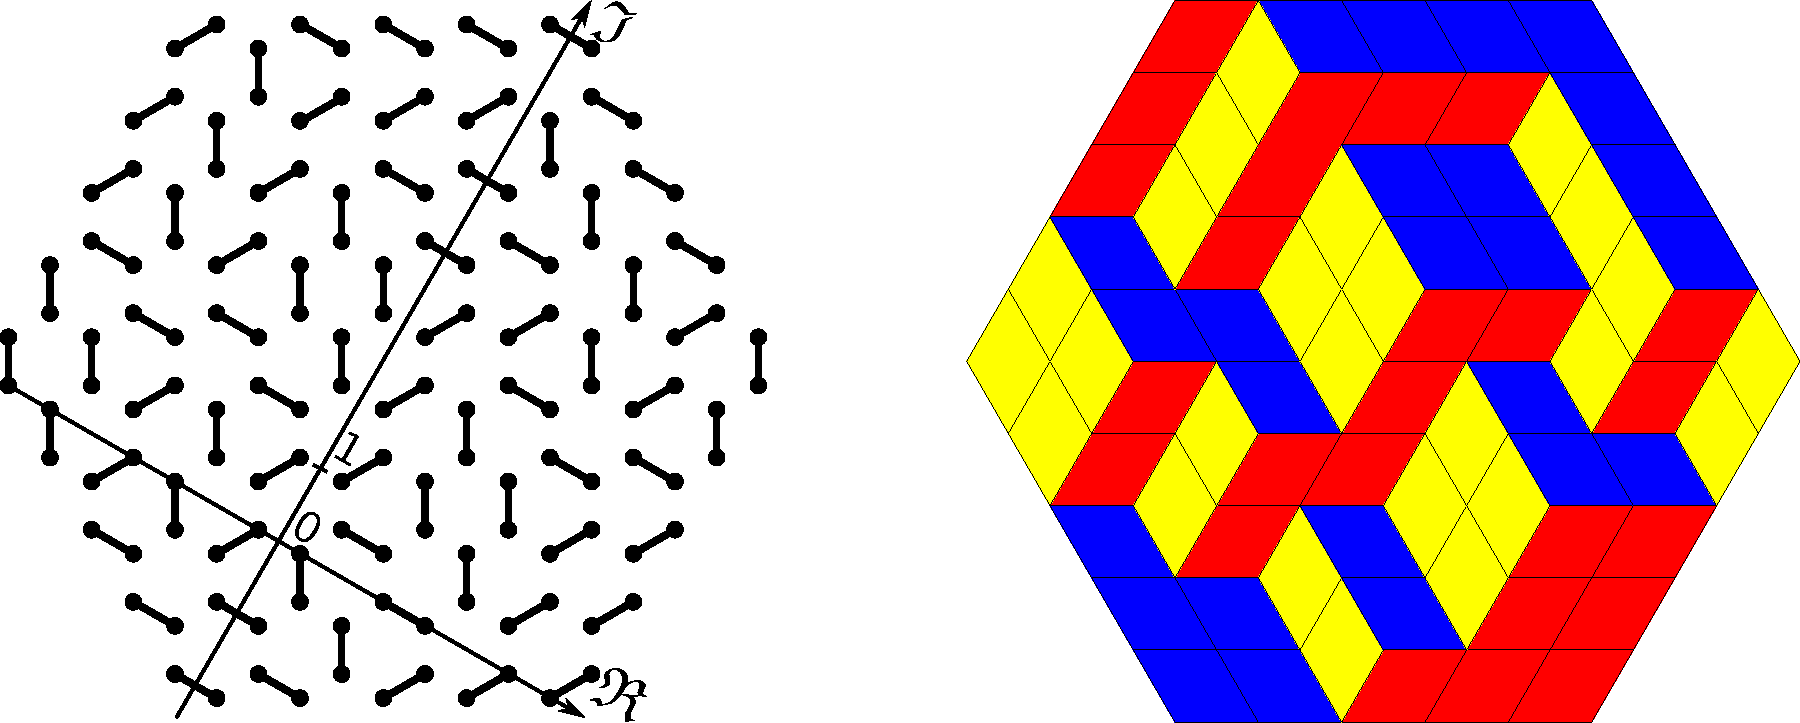
\includegraphics{my-loz}}}
\caption{\label{dhf}Слева: конфигурация димеров на шестиугольной решетке и выбор координат для
  определения весов  (\ref{eq:18}). Справа: соответствующая картина ``кубиков в углу коробки'' для
  функции высоты $h$.}
\end{figure}

Обозначим длины сторон шестиугольной области через $M$, $N$, и $K$. 
Вышеприведенное описание функции высоты можно сделать более строгим, если поставить неотрицательные
числа не превосходящие  $K$ в ячейки прямоугольной таблицы размером  $M\times N$ таким образом, что
значение в любой ячейке не превосходит значений в  ячейках, находящихся слева и сверху от нее:
\begin{equation}
  \label{eq:1}
  h_{ij}\leq h_{i-1,j},\quad h_{ij}\leq h_{i,j-1}.
\end{equation}

Вес каждой конфигурации дается экспонентой объема всех кубиков или, что то же самое, суммы значений
функции высоты:  
\begin{equation*}
  \label{eq:10}
  E[conf]=\sum_{i,j} h_{ij}=\mathrm{Volume}
\end{equation*}
Мы полагаем постоянную Больцмана равной единице и выбираем систему единиц таким образом, что в
выражение для энергии не входит константа связи. Тогда статсумма равна
\begin{equation*}
  \label{eq:14}
  Z=\sum_{conf} e^{-\frac{E[conf]}{T}}=\sum_{conf}q^{\mathrm{Volume}[conf]}, 
\end{equation*}
где $q=\exp\left(-1/T\right)$ .

В данном случае, статсумму можно записать в виде классической комбинаторной формулы Макмагона
~\cite{vuletic2009generalization}
\begin{equation}
  \label{eq:12}
   Z[M,N,K,q]=\prod_{i=1}^{M}\prod_{j=1}^{N}\prod_{k=1}^{K}\frac{1-q^{i+j+k-1}}{1-q^{i+j+k-2}}.
\end{equation}

Удельная свободная энергия определим, как$^{*}$
\footnote{Для удобства мы опускаем множитель  $\frac{1}{T}$ в обычном определении свободной энергии.}
\begin{equation*}
  \label{eq:17}
  % \frac{f}{T}
  f=-\frac{1}{V}\ln Z(M,N,K,q).
\end{equation*}
Здесь $V$ -- это количество вершин, оно вдвое больше числа димеров и вдвое больше числа граней
кубиков:
\begin{equation}
  \label{eq:19}
  V=2(MN+NK+MK)=2(ab+bc+ca) \varepsilon^{-2}.
\end{equation}

Мы будем рассматривать скейлинговый предел, одновременно с термодинамическим пределом, в котором
$T\to \infty,$ и  $M,N,K\to \infty$ так, что отношения $\frac{M}{T}=a,\quad \frac{N}{T}=b, \quad
\frac{K}{T}=c$ остаются постоянными.  Далее мы используем величину $\varepsilon=\frac{1}{T}$,
которую можно рассматривать в качестве характерного размера модели, например, шага решетки при нашем
выборе системы единиц.

В следующем разделе мы вычислим асимптотическое разложение свободной энергии $f$ по $\varepsilon$ и
выведем независимые от  $\varepsilon$ явные выражения для первых коэффициентов этого разложения.
  
\section{Вычисление асимптотического разложения свободной энергии}
\label{sec:free-energy-scaling}
Начнем с подстановки формулы Макмагона \eqref{eq:12} в определение свободной энергии \eqref{eq:17} и получим
\begin{multline}
  \label{eq:20}
    %-\frac{f}{T}
    f=-\frac{1}{V}\ln Z =\\=- \sum_{i=1}^{M} \sum_{j=1}^{N} \sum_{k=1}^{K} \frac{1}{V}\left[
  \ln\left(1-e^{-\varepsilon (i+j+k-3)} e^{-2\varepsilon}\right) -\ln\left(1-e^{-\varepsilon
      (i+j+k-3)} e^{-\varepsilon}\right)\right].
\end{multline}
Надо заметить, что для конечного  $\varepsilon$ и каждого значения  $i,j,k$ логарифмы имеют вид
$\ln(1-x)$, где $0<x<1$. То есть мы можем представить логарифмы в виде степенных рядов по $x$ и получить
\begin{equation}
  \label{eq:7}
  f=-\sum_{i=1}^{M} \sum_{j=1}^{N} \sum_{k=1}^{K}\sum_{n=1}^{\infty}
  \frac{1}{V}\frac{1}{n}\left[-e^{-n\varepsilon (i+j+k-3)} e^{-2n\varepsilon}+e^{-n\varepsilon
      (i+j+k-3)} e^{-n\varepsilon}\right]. 
\end{equation}
Здесь ряд сходится абсолютно, поэтому мы можем поменять порядок суммирования и переписать свободную
энергию в виде
\begin{equation}
  \label{eq:37}
  f=-\sum_{n=1}^{\infty}
  \frac{1}{V}\frac{1}{n}e^{-n\varepsilon}\left(1-e^{-n\varepsilon}\right)\sum_{i=1}^{M}
  \sum_{j=1}^{N} \sum_{k=1}^{K}e^{-n\varepsilon (i+j+k-3)} .
\end{equation}
Тройная сумма теперь факторизуется в произведение трех сумм типа  $\sum_{i=0}^{M-1}e^{-n\varepsilon
  i}$, которые оказываются суммами геометрических прогрессий. Поэтому  $\sum_{i=0}^{M-1}e^{-n\varepsilon
  i}=\frac{1-e^{-Mn\varepsilon}}{1-e^{-n\varepsilon}}$, и мы получаем
\begin{equation}
  \label{eq:38}
  f=-\sum_{n=1}^{\infty}
  \frac{1}{V}\frac{1}{n}\frac{e^{-n\varepsilon}}{\left(1-e^{-n\varepsilon}\right)^{2}}
  \left(1-e^{-na}\right)\left(1-e^{-nb}\right)\left(1-e^{-nb}\right).
\end{equation}
Обозначим через  $\chi(z)$ функцию
\begin{equation}
  \label{eq:39}
  \chi(z)=e^{-z}\left(\frac{z}{1-e^{-z}}\right)^{2}, 
\end{equation}
а через  $H_{n}$ произведение независящих от $\varepsilon$ экспонент
\begin{equation}
  \label{eq:40}
  H_{n}=\left(1-e^{-na}\right)\left(1-e^{-nb}\right)\left(1-e^{-nc}\right).
\end{equation}

Функция  $\chi(z)$ гладкая в 0, четная и имеет следующее разложение в ряд Тейлора:
\begin{equation}
  \label{eq:45}
  \chi(z)=1 - \frac{z^2}{12} + \frac{z^4}{240}+\mathcal{O}(z^{6}).
\end{equation}

Воспользуемся определением объема \eqref{eq:19} и запишем свободную энергию в виде
\begin{equation}
  \label{eq:41}
  f=-\frac{1}{2(ab+bc+ca)} \sum _{n=1}^{\infty} \frac{\chi(n\varepsilon)}{n^{3}} H_{n}.
\end{equation}
Мы интересуемся скейлинговым поведением по  $\varepsilon$, когда $\varepsilon\to 0$. Функция  $f$
регулярна по  $\varepsilon$ при $\varepsilon>0$. Поэтому нам необходимо вычислить
$\left.f\right|_{\varepsilon\to 0}$ и производные  $\left.\frac{\partial f}{\partial
  \varepsilon}\right|_{\varepsilon\to 0}$, $\left.\frac{\partial^{2} f}{\partial
  \varepsilon^{2}}\right|_{\varepsilon\to 0}$.

Для $\left.f\right|_{\varepsilon\to 0}$ мы видим, что $\chi(0)=1$, а сумма $\sum_{n=1}^{\infty}
\frac{H_{n}}{n^{3}}$ представляет собой сумму полилогарифмов
$\mathrm{Li}_{s}(z)=\sum_{n=1}^{\infty}\frac{z^{n}}{n^{s}}$ третьего порядка:
\begin{multline}
  \label{eq:42}
  \left.f\right|_{\varepsilon\to 0} =\frac{1}{2(ab+bc+ca)}\left[\Li_{3}(e^{-a})+\Li_{3}(e^{-b})+\Li_{3}(e^{-c})-
    \Li_{3}(e^{-a-b})\right.\\
  \left.-\Li_{3}(e^{-b-c})-    \Li_{3}(e^{-a-c})+    \Li_{3}(e^{-a-b-c})-\zeta(3)\right].
\end{multline}
Здесь дзета-функция Римана возникает, как значение полилогарифма $\Li_{3}(1)=\zeta(3)$.

Прозиводная функции $\chi(z)$ равна нулю, $\chi'(0)=0$, а ряды
$\sum_{n=1}^{\infty} \frac{\chi'(n\varepsilon)}{n^{2}}H_{n}$ сходятся при конечных значениях
$\varepsilon$, поэтому мы получаем для производной
\begin{equation}
  \label{eq:43}
\left.\frac{\partial f}{\partial \varepsilon}\right|_{\varepsilon\to 0}=0.
\end{equation}

Теперь вычислим вторую производную
\begin{equation}
  \label{eq:44}
\frac{\partial^{2} f}{\partial
  \varepsilon^{2}}=-\frac{1}{2(ab+bc+ca)} \sum _{n=1}^{\infty} \frac{\chi''(n\varepsilon)}{n} H_{n}.  
\end{equation}
Вторая производная  $\chi$ конечна,  $\chi''(0)=-\frac{1}{6}$. Но при переходе к пределу
$\varepsilon\to 0$ в этом выражении возникает сложность из-за плохой сходимости ряда. Перепишем
вторую производную в виде суммы двух рядов:
\begin{equation}
  \label{eq:46}
\frac{\partial^{2} f}{\partial
  \varepsilon^{2}}=-\frac{1}{2(ab+bc+ca)} \left(\sum _{n=1}^{\infty} \frac{\chi''(n\varepsilon)}{n}+
  \sum_{n=1}^{\infty} \frac{\chi''(n\varepsilon)}{n}(H_{n}-1)\right).    
\end{equation}
Вторая сумма теперь сходится, так как  $H_{n}-1$ экспоненциально убывает по $n$. Ее можно записать в
виде комбинации рядов для логарифмов:
\begin{multline}
  \label{eq:47}
  \chi''(0)\sum_{n=1}^{\infty} \frac{H_{n}-1}{n}=\\=\chi''(0)\sum_{n=1}^{\infty}\frac{1}{n}\left(-e^{-a
      n-b n-c n}+e^{-a n-b n}+e^{-a n-c n}+e^{-b n-c n} - e^{-a n}-e^{-b n}-e^{-c n}\right)=\\
  =\frac{1}{6}\ln\left(\frac{(e^{a}-1)(e^{b}-1)(e^{c}-1)(e^{a+b+c}-1)}{(e^{a+b}-1)(e^{b+c}-1)(e^{a+c}-1)}\right).
%%  =\frac{1}{6} \left(-\log \left(1-e^{-a-b-c}\right)+\log
%%   \left(1-e^{-a-b}\right)+\log
%%   \left(1-e^{-a-c}\right)+\log
%%   \left(1-e^{-b-c}\right)-\log
%%   \left(1-e^{-a}\right)-\log
%%   \left(1-e^{-b}\right)-\log
%%   \left(1-e^{-c}\right)\right)
\end{multline}

Первую сумму в формуле  \eqref{eq:46} можно выразить следующим образом. Во-первых, рассмотрим вторую
производную функции $\chi(z)$, выделим экспоненту и обозначим то, что осталось, через $\xi(z)$:
\begin{equation}
  \label{eq:48}
  \chi''(z)=e^{-z}\frac{e^{2 z} \left(z^2+4 e^z
   \left(z^2-1\right)+e^{2 z} \left(z^2-4
   z+2\right)+4
   z+2\right)}{\left(e^z-1\right)^4}=e^{-z}\xi(z).
\end{equation}
Сумму теперь можно переписать в виде
\begin{equation}
  \label{eq:49}
  \sum _{n=1}^{\infty} \frac{\chi''(n\varepsilon)}{n}=
  \sum_{n=1}^{\infty}\frac{e^{-n\varepsilon}}{n}\xi(n\varepsilon) =
  \sum_{n=1}^{\infty}\frac{e^{-n\varepsilon}}{n}\xi(0)+  \varepsilon\sum_{n=1}^{\infty}e^{-n\varepsilon}\frac{\xi(n\varepsilon)-\xi(0)}{n\varepsilon}.
\end{equation}
Первый член -- это ряд для логарифма $\ln\left(1-e^{-\varepsilon}\right)\approx \ln
\varepsilon$. Обозначим через  $Q(z)$ разность значений функции $\xi$ в $z$ и в нуле, деленную на $z$:
\begin{equation}
  \label{eq:85}
  Q(z)=\frac{\xi(z)-\xi(0)}{z}.
\end{equation}
Тогда функция  $Q(z)$ будет аналитической по $z$.

В результате вторая сумма может быть приближена интегралом:
\begin{equation}
  \label{eq:50}
  \varepsilon\sum_{n=1}^{\infty}e^{-n\varepsilon}Q(n\varepsilon)=\varepsilon\sum_{n=1}^{\infty}e^{-n\varepsilon}\frac{\xi(n\varepsilon)-\xi(0)}{n\varepsilon}\approx
  \int_{0}^{\infty} e^{-z}\frac{\xi(z)-\xi(0)}{z} dz=\int_{0}^{\infty}e^{-z}Q(z)\dz.
\end{equation}
\begin{equation}
  \label{eq:51}
  \frac{\partial^{2} f}{\partial
  \varepsilon^{2}}\approx-\frac{1}{2(ab+bc+ca)}
\left[\frac{1}{6}\ln\left(\frac{(e^{a}-1)(e^{b}-1)(e^{c}-1)(e^{a+b+c}-1)}{(e^{a+b}-1)(e^{b+c}-1)(e^{a+c}-1)}\right)-\frac{1}{6}\ln \varepsilon+\int_{0}^{\infty} e^{-z}\frac{\xi(z)-\xi(0)}{z} dz\right].
\end{equation}
Так как во вторую производную входит логарифмический член, мы получаем следующее поведение свободной энергии
\begin{equation}
  \label{eq:26}
  f\approx f_{0}+f_{1}\varepsilon +f_{2}\varepsilon^{2}\ln\varepsilon+ f_{3}\varepsilon^{2}+\mathcal{O}(\varepsilon^{3}),
\end{equation}
как и ожидается в двумерных критических системах  \cite{cardy1988finite}. После взятия производных
от этого выражения по  $\varepsilon$, мы видим, что
$f_{0}=f(0)$,$f_{1}=\left.\frac{\partial f}{\partial \varepsilon}\right|_{\varepsilon\to 0}$,
$\frac{\partial^{2} f}{\partial \varepsilon^{2}}=f_{2}(2\ln\varepsilon+3)+2f_{3}$. 

Таким образом мы получаем коэффициенты
\begin{multline}
  \label{eq:27}
  f_{0}=\frac{1}{2(ab+bc+ca)}\left[\Li_{3}(e^{-a})+\Li_{3}(e^{-b})+\Li_{3}(e^{-c})-
    \Li_{3}(e^{-a-b})\right.\\
  \left.-\Li_{3}(e^{-b-c})-    \Li_{3}(e^{-a-c})+    \Li_{3}(e^{-a-b-c})-\zeta(3)\right],
\end{multline}
\begin{equation}
  \label{eq:28}
  f_{1}=0,
\end{equation}
\begin{equation}
  \label{eq:30}
  f_{2}=-\frac{1}{2(ab+bc+ca)}\frac{1}{12},
\end{equation}
и
\begin{equation}
  \label{eq:29}
  f_{3}=-\frac{1}{2(ab+bc+ca)}\left[\frac{1}{12}\ln\left(\frac{(e^{a}-1)(e^{b}-1)(e^{c}-1)(e^{a+b+c}-1)}{(e^{a+b}-1)(e^{b+c}-1)(e^{a+c}-1)}\right)-\frac{1}{8}+ \frac{1}{2}\int_{0}^{\infty} e^{-z}Q(z) dz
    \right].
\end{equation}



\section{Предельная форма и физический смысл коэффициентов разложения}
\label{sec:accur-expans-phys}

В работе  \cite{1742-6596-1135-1-012024} мы представили результаты симуляции методами Монте-Карло,
использующими алгоритмы Метрополиса и Вонга-Ландау, которые подтверждают вид разложения
(\ref{eq:26}). В частности, мы получили $f_{1}=0.04\pm 0.04$, что согласуется со значением $f_{1}=0$. 

Димеры в скейлиноговом пределе в целом описываются теорией свободных фермионов
\cite{dijkgraaf2009dimer}, но на шестиугольной решетке (и на графах, допускающих существование
ориентации Кастелейна) модель переформулируется через функцию высоты, что можно рассматривать, как
бозонизацию теории \cite{gogolin2004bosonization}.

В скейлинговом пределе $\varepsilon\to 0$ в модели димеров возникает так называемая ``предельная форма''
~\cite{1998math......1068J,cohn1998shape}. Окрестности углов области ``заморожены'', значения
функции высоты на них фиксированы. Аналитическая ``арктическая кривая'' отделяет замороженные
области от области, где поведение описывается эффективной свободной теорией поля
\cite{kenyon2009lectures,kenyon2008height,kenyon2006dimers}. Более того, функция высоты в
скейлиноговом пределе стремится к определенной аналитической поверхности, а флуктуации вокруг этой
``предельной формы'' описываются свободной гауссовской теорией поля в искривленной фоновой метрике,
заданной ``предельной формой''. Можно использовать конформное отображение, чтобы перевести
внутренность ``арктической кривой'' в верхнюю полуплоскость.

Скейлиноговое поведение (\ref{eq:26}) логарифма статсуммы имеет вид, характерный для двумерных
моделей \cite{cardy1988finite}. 

Поэтому мы можем рассматривать первые два члена $f_{0}$ и $f_{1}$ как объемную и граничную свободную
энергию в соответствующей теории поля. Член $f_1$ отвечает вкладу ``предельной формы''. Так как у
нас детерминистическая замороженная граница, мы естественно видим, что $f_{1}=0$.
%The value of the first term $f_{0}$ can be rewritten using polylogarithm functions as

Член, пропорциональный логарифму характерной длины $\varepsilon$ также универсален
\cite{cardy1988finite} и должен возникать во всех двумерных теориях с границей. В статье
\cite{cardy1988finite} Карди и Пешель утверждают, что на гладком многообразии с характерной длиной
$L$ и с гладкой границей этот член должен иметь следующий вид:
\begin{equation}
  \label{eq:31}
  \delta F = -\frac{1}{6}{\bf c} \chi \ln L,
\end{equation}
где  ${\bf c}$ -- центральный заряд эффективной теории поля, а $\chi$ -- эйлерова характеристика
многообразия  $\chi=2-2 h-b$, где  $h$ -- количество ручек, а  $b$ -- число границ. Наивное
применение формулы  \eqref{eq:31} к нашему результату $\delta F=\frac{1}{12}$ дало бы ${\bf
  c}=\frac{1}{2}$, но это некорректно, так как мы должны рассматривать теорию поля в искривленной
фоновой метрике.

В случае наличия угловой сингулярности с углом $\Theta$ на границе, логарифмический вклад в
свободную энергию превращается в 
\begin{equation}
  \label{eq:86}
  \delta F = \frac{{\bf c}}{24}\left(\frac{\Theta}{\pi}-\frac{\pi}{\Theta}\right) \ln L.
\end{equation}
Эта формула недавно использовалась в работе Н. Аллегра \cite{allegra2015exact}, чтобы показать, что
центральный заряд при описании модели димеров в терминах функции высоты на квадратной решетке с
мономером в углу равняется единице ${\bf c}=1$, вопреки предыдущим работам, утверждавшим, что ${\bf
  c}=-2$ \cite{morin2016integrability}. 

В случае многообразия с конической сингулярностью с полу-углом $\Theta$, логарифмический вклад,
приведенный в работе \cite{cardy1988finite}, равен
\begin{equation}
  \label{eq:91}
  \delta F = \frac{{\bf c}}{24}\left(\frac{\Theta}{\pi}-\frac{4\pi}{\Theta}\right) \ln L.
\end{equation}

В нашем случае мы рассматриваем $2(ab+bc+ca)$ в качестве объема области, то есть
\begin{equation}
  \label{eq:33}
  \delta F = \left(2(ab+bc+ca)\right) f_{2}\ln\varepsilon.
\end{equation}

Применяя описанные выше формулы Карди и Пешеля, должно быть возможно вычислить  $\delta F$ через
значение центрального заряда для гауссовой свободной теории поля ${\bf c}=1$, кривизну метрики,
индуцированной предельной формой и конформное отображение из внутренней области ``арктической
кривой'' в верхнюю полуплоскость. Но метрика становится сингулярной у границы внутренней области
\cite{kenyon2007limit}, и вклад сингулярностей в логарифмическую поправку еще не изучен. Поэтому наш
результат для  $f_2$ должен быть полезен для такого исследования, которое мы постараемся представить
в отдельной публикации.

Последний член $f_{3}$ зависит только от формы области через $a,b,c$, с универсальным вкладом,
который равен интегралу функции  $e^{-z}\frac{\xi(z)-\xi(0)}{z}$. В следующих разделах мы покажем,
что эта константа возникает при устранении логарифмической расходимости даже для весов Больцмана,
зависящих от координаты.

\section{Численная проверка}
\label{sec:numeric-checks}
Для численной проверки нашего результата \eqref{eq:26} нам нужно вычислить интеграл в  $f_{3}$.
Функция  $e^{-z}\frac{\xi(z)-\xi(0)}{z}$ непрерывная и гладкая, но при численном вычислении предела
$z\to 0$ требуется осторожность. Вычисляя интеграл численно при помощи Mathematica, мы получаем
\begin{equation}
  \label{eq:2}
  \int_{0}^{\infty}e^{-z}Q(z)\dz=\int_{0}^{\infty}e^{-z}\frac{\xi(z)-\xi(0)}{z} dz = -0.080842.%0.08084228607897521
\end{equation}

Асимптотическое разложение \eqref{eq:26} дает очень хорошее приближение для свободной энергии. На
Рис.~\ref{fig:approx-acc} мы показываем точные и приближенные значения для $f$, а на правой
панели демонстрируем, что невязка аппроксимации ведет себя как  $\mathcal{O}(\varepsilon^{4})$. 

\begin{figure}[htbp]
  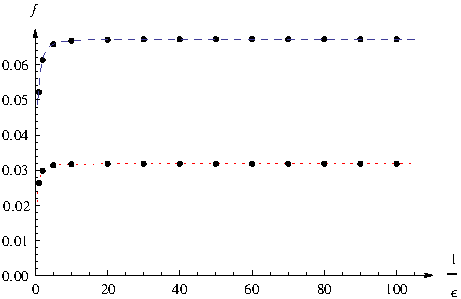
\includegraphics[scale=0.9]{exact-vs-approximation}
  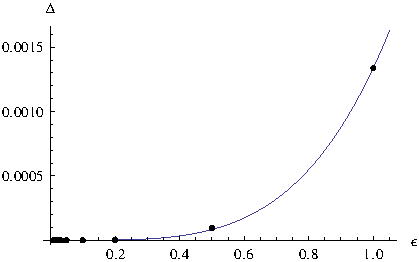
\includegraphics{error-1}
  \caption{\label{fig:approx-acc} {\it Слева:} Зависимость свободной энергии от  $1/\varepsilon$,
    вверху -- $a=b=c=1$, внизу -- $a=3, b=2, c=1$. Точные значения обозначены черными точками.
    Приближение по формуле  \eqref{eq:26} изображено голубой и красной пунктирными линиями.  {\it
      Справа:} Зависимость невязки аппроксимации от $\varepsilon$, сплошная линия -- приближение
    функцией $b\varepsilon^{4}$.}
\end{figure}

\section{Коробка бесконечной высоты}
\label{sec:gener-other-doma}

Рассмотрим случай кубиков в коробке бесконечной высоты. В этом случае $K=\infty$, а  $M,N$ --
конечны. Теперь шестиугольная область конфигураций димеров имеет сторону бесконечной длины, и общее
число димеров бесконечно, поэтому более естественно полагать объем системы равным $V=MN$.  

Положив $K=\infty$ в статсумме, мы видим, что все члены с  $k$ сокращаются и остается 
\begin{equation}
  \label{eq:3}
  Z[M,N,q]=\prod_{i=1}^{M}\prod_{j=1}^{N}\frac{1}{1-q^{i+j-1}}.
\end{equation}

Вычисление свободной энергии практически полностью повторяет вычисление в случае коробки конечной
высоты. Мы раскладываем логарифм в выражении для свободной энергии, а затем факторизуем сумму:
\begin{multline}
  \label{eq:4}
  f=-\frac{1}{MN}\sum_{i=1}^{M}\sum_{j=1}^{N}\ln\left(1-e^{-\varepsilon(i+j-2)}e^{-\varepsilon}\right)=\\
  =\sum_{n=1}^{\infty}\frac{\varepsilon^{2}}{ab}\frac{1}{n}e^{-n\varepsilon}\left(\sum_{i=1}^{M}e^{-n\varepsilon(i-1)}\right)
  \left(\sum_{j=1}^{N}e^{-n\varepsilon(j-1)}\right).
\end{multline}
Вычисляя суммы геометрических прогрессий, мы получаем почти такие же выражения, как в формуле
\eqref{eq:38}, за исключением того, что $H_{n}$ теперь содержит только два множителя $H_{n}
=\left(1-e^{-na}\right)\left(1-e^{-nb}\right)$: 
\begin{equation}
  \label{eq:5}
  f=-\frac{1}{ab} \sum_{n=1}^{\infty}\frac{\chi(n\varepsilon)}{n^{3}} H_{n}.
\end{equation}
Функция  $\chi(z)=e^{-z}\left(\frac{z}{1-e^{-z}}\right)^{2}$ та же, что и в формуле \eqref{eq:39}. 

Повторяя вычисления из раздела  \ref{sec:free-energy-scaling}, мы получаем следующие результаты для
коэффициентов $f_{0}, f_{1}, f_{2}, f_{3}$: 
\begin{equation}
  \label{eq:6}
  f_{0}=\frac{1}{ab}\left[\Li_{3}(e^{-a})+\Li_{3}(e^{-b})-
    \Li_{3}(e^{-a-b})-\zeta(3)\right],
\end{equation}
\begin{equation}
  \label{eq:8}
  f_{1}=0,
\end{equation}
\begin{equation}
  \label{eq:9}
  f_{2}=\frac{1}{ab}\frac{1}{12},
\end{equation}
\begin{equation}
  \label{eq:11}
  f_{3}=-\frac{1}{ab}\left[\frac{1}{12}\ln\left(\frac{(e^{a}-1)(e^{b}-1)}{(e^{a+b}-1)}\right)-\frac{1}{8}+ \frac{1}{2}\int_{0}^{\infty} e^{-z}\frac{\xi(z)-\xi(0)}{z} dz
    \right].
\end{equation}

В этом случае мы так же видим на Рис.~\ref{fig:approx-acc-2d} хорошее численное совпадение
асимптотического разложения \eqref{eq:26} и точной формулы  \eqref{eq:4}. 

Так как шестиугольник с бесконечной стороной похож на бесконечную полосу, естественно сравнить наш
результат с результатами для поправок конечного размера к скейлингу свободной энергии в модели
димеров на квадратной решетке на полосе, цилиндре и полосе, замкнутой в ленту Мёбиуса. Такие
результаты были недавно собраны вместе в работе \cite{izmailian2017finite}, а в работе
\cite{Sh_Izmailian_2019} был проведен их дальнейший анализ. В этих работах предложено следующее
общее выражение для разложения свободной энергии на квадратной решетке размером $M\times N$ (здесь
$S=M\times N$ ): 
\begin{equation}
  \label{eq:32}
  f=f_{\mathrm{bulk}}+\frac{2}{M}f_{s1}+\frac{2}{N}f_{s2}
  +f_{\mathrm{corn}}\frac{\ln S}{S} +\frac{1}{S} (f_{\mathrm{univ}}+f_{\mathrm{nonuniv}})
\end{equation}
В частности, на полосе объемный член $f_{\mathrm{bulk}}=\frac{G}{\pi}$, где  $G$ -- константа
Каталана, поверхностная свободная энергия отлична от нуля $f_{s1}=-\frac{1}{4}\ln(1+\sqrt{2})$, а
коэффициент перед  $\frac{1}{S}$ равен  $\frac{\pi}{24}$. В случае цилиндра и полосы Мёбиуса
логарифмический член также присутствует. 

Сравнивая наши результаты \eqref{eq:6}, \eqref{eq:8}, \eqref{eq:9}, \eqref{eq:11} с этими
выражениями, мы видим, что поведение на шестиугольной решетке в присутствии предельной формы
отличается. В частности, объемный член $f_{0}$ зависит от геометрических параметров $a$ и  $b$,
граница свободна от натяжения, так что граничный член $f_{1}$ равен нулю, и геометрические параметры
области также входят и в коэффициент при $\varepsilon^{2}$. 

\begin{figure}[htbp]
  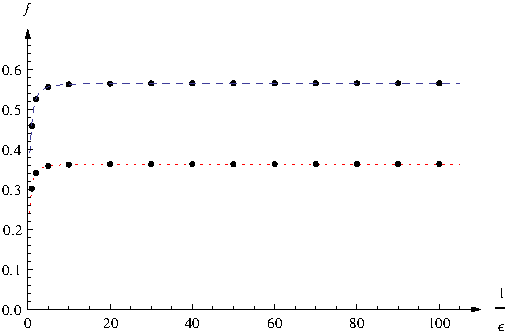
\includegraphics[scale=0.8]{exact-vs-approximation-2d}
  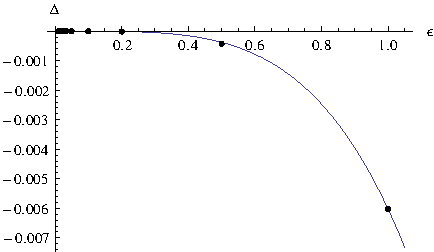
\includegraphics[scale=0.9]{error-2d}
  \caption{\label{fig:approx-acc-2d} {\it Слева:} Зависимость свободной энергии от  $1/\varepsilon$
    в коробке бесконечной высоты, вверху при $a=b=1$, внизу -- $a=2, b=1$. Точные значения показаны
    черными точками. Приближения при помощи формулы \eqref{eq:26} изображены синей и красной
    пунктирными линиями. {\it Справа:} Зависимость невязки аппроксимации от  $\varepsilon$, сплошная
    линия -- приближение функцией $b\varepsilon^{4}$.}
\end{figure}

\section{Коробка бесконечной высоты с весами Больцмана, зависящими от координаты}
\label{sec:box-infinite-height}

Рассмотрим теперь обобщение на случай, когда  $q$ зависит от координаты. Обычно полагают, что  $q$
принимает различные значения на диагоналях, которые нумеруются координатой $t$. Нам нужно ввести
некоторые обозначения, чтобы можно было рассматривать скейлинговый предел. Пусть  $\varphi(t)$ --
непрерывная ограниченная гладкая функция при  $t\in\left[-a,b\right]$. Введем обозначение
$q_{i}=e^{-\varepsilon \varphi\left(i\varepsilon\right)}$ при $i=(-M+1)\dots N-1$. Мы нумеруем
диагонали таким образом, что левый верхний угол прямоугольника $M\times N$ имеет номер $N-M$, правый
верхний -- $N$, левый нижний -- $-M$, а правый нижний -- $0$. (См. Рис. \ref{fig:box-t-coords}).
Диагонали с индексами  $N$ и $-M$ имеют нулевую длину, поэтому мы можем положить $q_{N}=q_{-M}=0$.
Всего у нас не более $N+M-1$ непустой диагонали. 

\begin{figure}[htbp]
  \includegraphics[scale=0.5]{box-t-coords}
  \caption{\label{fig:box-t-coords} Координаты диагоналей.}
\end{figure}

Статсумма для этого и более общего случая произвольной формы внутренней границы коробки была
вычислена в работе  \cite{okounkov2007random}. В нашем случае она содержит произведения весов
$q_{i}$ для диагоналей с отрицательными и положительными номерами:
\begin{equation}
  \label{eq:13}
  Z=\prod_{i=0}^{N-1}\prod_{j=0}^{M-1} \frac{1}{1-q_{N-M}^{-1}\left(\prod_{k=0}^{i}q_{N-M-k}\right)\left(\prod_{l=0}^{j}q_{N-M+l}\right)}.
\end{equation}
(См. Теорему 2 в \cite{okounkov2007random}).
Если мы положим  $q_{i}=q$,  мы восстановим формулу \eqref{eq:3}.

Опять рассмотрим зависимость свободной энергии от $\varepsilon$:
\begin{equation}
  \label{eq:21}
  f=-\frac{\varepsilon^{2}}{ab}\sum_{i=0}^{N-1}\sum_{j=0}^{M-1}\ln
  \left(1-e^{\varepsilon \varphi(b-a)}e^{-\varepsilon\sum_{k=0}^{i}\varphi\left(b-a-k\varepsilon\right)}
    e^{-\varepsilon\sum_{l=0}^{j}\varphi\left(b-a+l\varepsilon\right)} \right).
\end{equation}

Член  $f_{0}$ в асимптотическом разложении  \eqref{eq:26} легко можно получить из этого выражения.
Для этого нам нужно приблизить суммы интегралами, воспользовавшись формулой
$\sum_{k=0}^{i}\varepsilon\varphi(b-a-k\varepsilon)\approx
\int_{0}^{i\varepsilon}\varphi(b-a-x)\dx$%%!!!!! Write more here
и аналогичными приближениями для других сумм:
\begin{multline}
  \label{eq:74}
  f_{0}=-\frac{1}{ab}\int_{0}^{b}\int_{0}^{a}\ln
  \left(1-e^{-\int_{0}^{y}\varphi\left(b-a-x\right)\dx}
    e^{-\int_{0}^{z}\varphi\left(b-a+\bar x\right)\dxb} \right)\dz\dy=\\
  =-\frac{1}{ab}\int_{0}^{b}\int_{0}^{a}\ln
  \left(1-e^{-\int_{-y}^{z}\varphi\left(b-a+x\right)\dx} \right)\dz\dy.
\end{multline}
Подставим в это выражение  $\varphi(x)\equiv 1$, мы немедленно получаем формулу \eqref{eq:6}, так
как полилогарифмы являются интегралами логарифмов. Хоть логарифм и расходится в точке $y=z=0$, эта
расходимость исчезает после двойного интегрирования. 

Для вычисления члена $f_{1}$ мы воспользуемся следующей простой леммой:
\begin{lemma}
  Пусть  $a=M\varepsilon$ и $b=N\varepsilon$.
  Для интегрируемой почти всюду аналитической функции  $f$ и аналитической функции $\varphi$ сумма
  может быть приближена интегралом с поправками порядка $o(\varepsilon)$:
  \begin{equation}
    \label{eq:75}
    \sum_{i=0}^{M-1}\sum_{j=0}^{N-1}\varepsilon^{2}f\left(\varepsilon\sum_{k=-i}^{j}\varphi(k\varepsilon)\right)=
    \int_{0}^{a}\int_{0}^{b}f\left(\int_{-y}^{z}\varphi(x)\dx\right)\dz\;\dy+o(\varepsilon).
  \end{equation}
  \begin{proof}
    Воспользуемся формулой Эйлера-Маклорена для приближения сумм интегралами с поправками.
    Достаточно рассмотреть линейные по $\varepsilon$ члены. Сперва используем формулу для первой
    суммы в аргументе функции $f$:
  \begin{equation}
    \label{eq:76}
    \sum_{i=0}^{M-1}\sum_{j=0}^{N-1}\varepsilon^{2}f\left(\varepsilon\sum_{k=-i}^{j}\varphi(k\varepsilon)\right)=
    \sum_{i=0}^{M-1}\sum_{j=0}^{N-1}\varepsilon^{2}f\left(\int_{-i\varepsilon}^{j\varepsilon}\varphi(x)\dx+\frac{\varepsilon}{2}\left(\varphi(j\varepsilon)-\varphi(-i\varepsilon)\right)+\mathcal{O}(\varepsilon^{2})\right).
  \end{equation}
  Для двойной суммы можно использовать следующий простой аналог формулы Эйлера-Маклорена. Пусть $G$
  -- аналитическая функция на прямоугольнике  $[0,a]\times[0,b]$, тогда
\begin{equation}
  \label{eq:77}
  \int_{0}^{a} \int_{0}^{b}G(y,z) \dz\; \dy\;
  \approx\sum_{i=0}^{M-1}\sum_{j=0}^{N-1}\left\{\varepsilon^{2}G\left(i\varepsilon,j\varepsilon\right)+
    \frac{\varepsilon^{3}}{2}\left((\partial_{y}+\partial_{z})G\right)(i\varepsilon,j\varepsilon)\right\}+o(\varepsilon^{2}).
\end{equation}
Эта формула элементарно выводится путем разбиения области интегрирования на квадратики со стороной
$\varepsilon$ и подстановки рядов Тейлора для  $G$ в интегралы.

Обозначим через $G_{\varepsilon}(y,z)$ функцию двух аргументов, входящую в двойную сумму в \eqref{eq:76}:
\begin{equation}
  \label{eq:78}
  G_{\varepsilon}(y,z)=f\left(\int_{-y}^{z}\varphi(x)\dx+\frac{\varepsilon}{2}(\varphi(z)-\varphi(-y))+o(\varepsilon)\right).
\end{equation}
Используем формулу \eqref{eq:77}, чтобы выразить двойную сумму в формуле \eqref{eq:76} через
интеграл и поправку:
\begin{equation}
  \label{eq:79}
  \sum_{i=0}^{M-1}\sum_{j=0}^{N-1}\varepsilon^{2}G_{\varepsilon}(i\varepsilon,j\varepsilon)=\int_{0}^{a}\int_{0}^{b}
  G_{\varepsilon}(y,z)\dz\;\dy-
  \frac{\varepsilon^{3}}{2}
  \sum_{i=0}^{M-1}\sum_{j=0}^{N-1}\left((\partial_{y}+\partial_{z})G_{\varepsilon}\right)(i\varepsilon,j\varepsilon)+o(\varepsilon^{3}).
\end{equation}
Теперь разложим функцию $G_{\varepsilon}(y,z)$ под интегралом в ряд Тейлора по $\varepsilon$:
\begin{equation}
  \label{eq:80}
  \int_{0}^{a}\int_{0}^{b}G_{\varepsilon}(y,z)\dz\;\dy=
  \int_{0}^{a}\int_{0}^{b}G_{0}(y,z)\dz\;\dy+\int_{0}^{a}\int_{0}^{b}\frac{\varepsilon}{2}(\varphi(z)-\varphi(-y))\cdot
  f'\left(\int_{-y}^{z}\varphi(x)\dx\right)\dz\;\dy+o(\varepsilon). 
\end{equation}
С другой стороны, производные  $G_{\varepsilon}$ по  $y,z$ вычисляются как
\begin{eqnarray}
  \label{eq:81}
  \partial_{z}G_{\varepsilon}(y,z)=f'\left(\int_{-y}^{z}\varphi(x)\dx+\frac{\varepsilon}{2}(\varphi(z)-\varphi(-y))+o(\varepsilon)\right)\varphi(z)+o(\varepsilon)\\ 
  \partial_{y}G_{\varepsilon}(y,z)=-f'\left(\int_{-y}^{z}\varphi(x)\dx+\frac{\varepsilon}{2}(\varphi(z)-\varphi(-y))+o(\varepsilon)\right)\varphi(-y)+o(\varepsilon).
\end{eqnarray}
Подставляя равенства  \eqref{eq:80},\eqref{eq:81} в  \eqref{eq:79} и используя формулу \eqref{eq:77}
для замены двойной суммы производных  $G_{\varepsilon}$ на двойной интеграл, мы видим, что линейные
поправки по  $\varepsilon$ сокращаются. 
\end{proof}
\end{lemma}

Воспользуемся леммой для нашей удельной свободной энергии $f$, которая является аналитической
функцией, и для нашей гладкой функции  $\varphi$. Мы немедленно получаем, что
\begin{equation}
  \label{eq:82}
  f_{1}=0.
\end{equation}

Следующие члены асимптотического разложения требуют больших усилий, так как мы должны выделить вклад
порядка $\varepsilon^{2}\ln\varepsilon$. 

Поэтому для вывода выражений для высших порядков в разложении \eqref{eq:26} нам нужно разложить
логарифм, поменять порядок суммирования и переписать свободную энергию таким же образом, как мы
делали это ранее:
\begin{equation}
  \label{eq:22}
   f=\sum_{n=1}^{\infty}\frac{\varepsilon^{2}}{ab}\frac{1}{n}e^{n\varepsilon
     \varphi(b-a)}\sum_{i=0}^{N-1}\sum_{j=0}^{M-1} e^{-n\varepsilon\sum_{k=0}^{i}\varphi\left(b-a-k\varepsilon\right)}
    e^{-n\varepsilon\sum_{l=0}^{j}\varphi\left(b-a+l\varepsilon\right)}.
  \end{equation}
Мы снова факторизуем двойную сумму в произведение двух сумм:  
\begin{equation}
  \label{eq:23}
    f=\sum_{n=1}^{\infty}\frac{\varepsilon^{2}}{ab}\frac{1}{n}e^{-n\varepsilon
     \varphi(b-a)}\left(\sum_{i=0}^{N-1}
     e^{-n\varepsilon\sum_{k=1}^{i}\varphi\left(b-a-k\varepsilon\right)}\right)
   \left(\sum_{j=0}^{M-1}e^{-n\varepsilon\sum_{l=1}^{j}\varphi\left(b-a+l\varepsilon\right)}\right),
 \end{equation}
 где мы полагаем, что $\sum_{k=1}^{0}\varphi(b-a-k\varepsilon)=0$ и
$\sum_{l=1}^{0}\varphi(b-a+l\varepsilon)=0$. Заметим, что при  $\varphi(t)\equiv 1$ мы восстановим формулу
\eqref{eq:4}.

Введем следующие обозначения:
\begin{equation}
  \label{eq:52}
  r_{\mp}(i\varepsilon)\equiv\varepsilon\sum_{k=1}^{i}\varphi(b-a\mp k\varepsilon).
\end{equation}
Функции  $r_{\mp}$ могут быть приближены по формуле Эйлера-Маклорена следующим образом:
\begin{equation}
  \label{eq:53}
  r_{\mp}(x)\approx\int_{0}^{x}\varphi(b-a\mp y) \dy +\frac{\varepsilon}{2}\left(\varphi(b-a\mp
    x)-\varphi(b-a)\right)\mp \frac{\varepsilon^{2}}{12}\left(\varphi'(b-a\mp x)-\varphi'(b-a)\right).
\end{equation}
Обозначим через $\Psi_{n}^{\mp}$ следующие функции:
\begin{equation}
  \label{eq:54}
  \Psi^{\mp}_{n}(x)\equiv e^{-nr_{\mp}(x)}-e^{-nxr_{\mp}'(0)}.
\end{equation}
Эти функции аналитичны по  $\varepsilon$, кроме того, высшие производные  $\Psi^{\mp}_{n}$ растут по
$n$ не слишком быстро. Поэтому суммы рядов, записанных через эти функции и их производные, сходятся,
как мы увидим далее. 

С такими обозначениями мы можем записать свободную энергию в виде
\begin{multline}
  \label{eq:55}
  f=\frac{1}{ab}\sum_{n=1}^{\infty}\frac{1}{n}e^{-n\varepsilon\varphi(b-a)}\left[\varepsilon^{2}\sum_{i=0}^{N-1}e^{-n\varepsilon
    i r_{-}'(0)}\sum_{j=0}^{M-1}e^{-n\varepsilon j
    r_{+}'(0)}+\varepsilon\sum_{i=0}^{N-1}e^{-n\varepsilon i
    r_{-}'(0)}\varepsilon\sum_{j=0}^{M-1}\Psi^{+}_{n}(j\varepsilon)+\right.\\
\left. +\varepsilon\sum_{i=0}^{N-1}\Psi^{-}_{n}(i\varepsilon) \cdot\varepsilon\sum_{j=0}^{M-1}e^{-n\varepsilon
  j r_{+}'(0)}+\varepsilon\sum_{i=0}^{N-1}\Psi^{-}_{n}(i\varepsilon)
\cdot\varepsilon\sum_{j=0}^{M-1}\Psi^{+}_{n}(j\varepsilon)\right]=\\
=f^{(0)}+f^{+}+f^{-}+f^{\times}.
\end{multline}
Первый член $f^{(0)}$ можно явно вычислить:
\begin{equation}
  \label{eq:56}
  f^{(0)}=\frac{1}{ab}\sum_{n=1}^{\infty}\frac{1}{n} e^{-n\varepsilon
    \varphi(b-a)}\varepsilon^{2}\frac{\left(1-e^{-n b r_{-}'(0)}\right)\left(1-e^{-n a
        r_{+}'(0)}\right)}{\left(1-e^{-n\varepsilon r_{-}'(0)}\right)\left(1-e^{-n\varepsilon r_{+}'(0)}\right)}.
\end{equation}

Обозначим числитель этого выражения $H_{n}(\varepsilon)$:
\begin{equation}
  \label{eq:57}
  H_{n}(\varepsilon)=\left(1-e^{-n b r_{-}'(0)}\right)\left(1-e^{-n a r_{+}'(0)}\right).
\end{equation}
Заметим, что
\begin{equation}
  \label{eq:58}
  r_{\mp}'(0)=\varphi(b-a)\mp \frac{\varepsilon}{2} \varphi'(b-a)+\frac{\varepsilon^{2}}{12} \varphi''(b-a)+\mathcal{O}(\varepsilon^{3}).
\end{equation}
можно переписать в виде
\begin{equation}
  \label{eq:59}
  r_{\mp}'(0)=\varphi(b-a)\left(1+\alpha_{\mp}(\varepsilon)\right), 
\end{equation}
где
\begin{equation}
  \label{eq:60}
  \alpha_{\mp}(\varepsilon)=\mp
  \frac{\varepsilon}{2}\frac{\varphi'(b-a)}{\varphi(b-a)}+\frac{\varepsilon^{2}}{12} \frac{\varphi''(b-a)}{\varphi(b-a)}+\mathcal{O}(\varepsilon^{3}).
\end{equation}

Теперь для $f^{(0)}$ у нас получается
\begin{equation}
  \label{eq:61}
  f^{(0)}=\frac{1}{ab}\sum_{n=1}^{\infty} \frac{\tilde{\chi}_{n}\left(n\varepsilon
      \varphi(b-a),\varepsilon\right) }{n^{3}\varphi(b-a)^{2}},
\end{equation}
где $\tilde{\chi}_{n}(z,\varepsilon)$ определена как
\begin{equation}
  \label{eq:62}
  \tilde{\chi}_{n}(z,\varepsilon)\equiv \frac{z^{2} e^{-z}
    H_{n}(\varepsilon)}{\left(1-e^{-z\left(1+\alpha_{-}(\varepsilon)\right)}\right)
    \left(1-e^{-z\left(1+\alpha_{+}(\varepsilon)\right)}\right)}.
\end{equation}
Важно включить сюда $H_{n}(\varepsilon)$, так как $H_{n}(\varepsilon)$ содержит убывающие экспоненты
по $n$.

Вычисляя производные  $f^{(0)}$ по $\varepsilon$, мы получаем
\begin{multline}
  \label{eq:63}
  \left(\frac{d}{d\varepsilon}\right)^{2} f^{(0)}=\frac{1}{ab\varphi(b-a)} \sum_{n=1}^{\infty}
  \frac{1}{n^{3}}\left[
    \left.\tilde{\chi}''_{n,\varepsilon\varepsilon}\left(n\varepsilon\varphi(b-a),\varepsilon\right)\right|_{\varepsilon=0}+
    2n\varphi(b-a)\left.\tilde{\chi}''_{n,z\varepsilon}\left(n\varepsilon\varphi(b-a),\varepsilon\right)\right|_{\varepsilon=0}+\right.\\\left.
      n^{2}\left(\varphi(b-a)\right)^{2}\tilde{\chi}''_{n,zz}\left(n\varepsilon\varphi(b-a),\varepsilon\right)  \right]+
    \mathcal{O}(\varepsilon \ln \varepsilon)=\\
    =\frac{1}{ab\varphi(b-a)}\left[\sum_{n=1}^{\infty} \frac{1}{n^{3}}
      \tilde{\chi}''_{n,\varepsilon\varepsilon}(0,0)+2\varphi(b-a)\sum_{n=1}^{\infty}\frac{1}{n^{2}}\tilde{\chi}''_{n,z\varepsilon}(0,0)\right]+
    \\
    +\frac{1}{ab}\sum_{n=1}^{\infty}\frac{H_{n}}{n}\chi''\left(n\varepsilon\varphi(b-a)\right)+\mathcal{O}(\varepsilon\ln \varepsilon),
\end{multline}
где функция  $\chi(z)$ та же, что и в равенстве \eqref{eq:39}
\begin{equation}
  \label{eq:64}
  \chi(z)=\frac{z^{2} e^{-z}}{\left(1-e^{-z}\right)^{2}}
\end{equation}
и
\begin{equation}
  \label{eq:65}
  H_{n}=\left(1-e^{-nb\varphi(b-a)}\right) \left(1-e^{-na\varphi(b-a)}\right).
\end{equation}

Последняя сумма в последней строке равенства \eqref{eq:63} такая же, как и в разделе
\ref{sec:gener-other-doma}, поэтому ее можно вычислить
\begin{multline}
  \label{eq:66}
  \frac{1}{ab}\sum_{n=1}^{\infty}\frac{H_{n}}{n}\chi''\left(n\varepsilon \varphi(b-a)\right)=
  \frac{1}{ab}\left(\frac{1}{6}\ln \varepsilon +\frac{1}{6}\ln \varphi(b-a)+ \int_{0}^{\infty}
    e^{-z}Q(z) \dz+\chi''(0)\sum_{n=1}^{\infty}\frac{H_{n}-1}{n}\right)=\\
  =\frac{1}{ab}\left(\frac{1}{6}\ln \varepsilon +\frac{1}{6}\ln \varphi(b-a)+ \int_{0}^{\infty}
    e^{-z}Q(z) \dz+\frac{1}{6}\ln\left(\frac{\left(1-e^{a\varphi(b-a)}\right)\left(1-e^{a\varphi(b-a)}\right)}{1-e^{(a+b)\varphi(b-a)}}\right)\right),
\end{multline}
где $Q(z)$ было определено в формуле \eqref{eq:85}.

В итоге вклад $f^{(0)}$ в асимптотическое разложение \eqref{eq:26} дается членом
\begin{equation}
  \label{eq:87}
f^{(0)}_{3}=\frac{1}{ab\varphi(b-a)}\left[\sum_{n=1}^{\infty} \frac{1}{n^{3}}
  \tilde{\chi}''_{n,\varepsilon\varepsilon}(0,0)+2\varphi(b-a)\sum_{n=1}^{\infty}\frac{1}{n^{2}}\tilde{\chi}''_{n,z\varepsilon}(0,0)\right],
\end{equation}
который имеет сложный вид, но не зависит от  $\varepsilon$ и может быть выписан явно, и выражением
\eqref{eq:66}, которое дает логарифмическое поведение по $\varepsilon$.

Теперь мы должны рассмотреть другие члены в выражении \eqref{eq:55}. Для $f^{+}$ получаем
\begin{equation}
  \label{eq:67}
  f^{+}=\frac{1}{ab}\sum_{n=1}^{\infty}\frac{1}{n} e^{-n\varepsilon\varphi(b-a)} \varepsilon
  \frac{1-e^{-nbr_{-}'(0)}}{1-e^{-n\varepsilon r_{-}'(0)}}\varepsilon\sum_{j=0}^{M-1}\Psi^{+}_{n}(j\varepsilon).
\end{equation}
Сумма по $j$ может быть приближена интегралом с помощью формулы Эйлера-Маклорена
\begin{equation}
  \label{eq:68}
  \varepsilon\sum_{j=0}^{M-1}\Psi^{+}_{n}(j\varepsilon) = \int_{0}^{a}\Psi^{+}_{n}(x) \dx -
  \frac{\varepsilon}{2}\left(\Psi^{+}_{n}(a)-\Psi^{+}_{n}(0)\right)+
  \frac{\varepsilon^{2}}{12}\left(\Psi^{+'}_{n}(a)-\Psi^{+}_{n}(0)\right)+
  \mathcal{O}\left(\varepsilon^{m}\Psi^{+(m-1)}_{n}\right).
\end{equation}
Так как функция $r(x)$ аналитическая и  $r(0)=0$, мы можем написать $r(x)=xr'(0)+x^{2}\zeta(x)$, поэтому
\begin{equation}
  \label{eq:83}
\Psi_{n}(x)=e^{-nr'(0)x}\left(e^{-n\left(r(x)-xr'(0)\right)}-1\right)=e^{-nxr'(0)}\left(e^{-nx^{2}\zeta(x)}-1\right)  
\end{equation}
и мы видим, что $\Psi_{n}(0)=0$ и $\Psi_{n}'(0)=0$.
Тогда в пределе $n\to\infty$ мы получаем
\begin{equation}
  \label{eq:69}
  \int_{0}^{c}\Psi_{n}(x)
  \dx \xrightarrow[n\to\infty]{}\int_{0}^{c}e^{-nxr'(0)}\left(-nx^{2}\zeta(x)+\dots\right)\dx\sim \frac{1}{n^{2}}.
\end{equation}
Производные  $\Psi$ ведут себя как  $\Psi_{n}^{(m)}(0)\sim n^{m-1}$, так как мы должны
дифференцировать выражение в скобках в формуле \eqref{eq:83}, чтобы получить ненулевое значение, а
тогда возникает дополнительная степень  $x$, которую тоже нужно дифференцировать. Поэтому вклад от
$\varepsilon^{m}\Psi_{n}^{(m-1)}(0)$ в $f^{+}$ дает
\begin{equation}
  \label{eq:70}
  \sum_{n=1}^{\infty} \frac{1}{n} e^{-n\varepsilon\varphi(b-a)}
  \frac{1-e^{-nbr_{-}'(0)}}{1-e^{-n\varepsilon r_{-}'(0)}} \varepsilon^{m+1}\Psi_{n}^{(m-1)}(0)\sim
  \sum_{n=1}^{\infty} \frac{1}{n^{4}} e^{-n\varepsilon\varphi(b-a)}
  \frac{1-e^{-nbr_{-}'(0)}}{1-e^{-n\varepsilon r_{-}'(0)}} (\varepsilon n )^{m+1}.
\end{equation}
Для второй производной по  $\varepsilon$ мы получаем, что основной вклад ведет себя как
$\sum_{n=1}\frac{1}{n^{2}}e^{-n\varepsilon\varphi(b-a)}
  (n\varepsilon)^{m+1}\xrightarrow[\varepsilon\to 0]{}0,$
если $m\geq 3$. Для членов с  $m=0,1,2$ нам нужно вычислить предел при $\varepsilon\to 0$. После
этого вычисления мы получаем:
\begin{multline}
  \label{eq:71}
  f^{+}_{3}\equiv\left.\left(\frac{d}{d\varepsilon}\right)^{2} f^{+}\right|_{\varepsilon=0} =\\
  \left.\left(\frac{d}{d\varepsilon}\right)^{2}\frac{1}{ab}\sum_{n=1}^{\infty} \frac{1}{n}
  e^{-n\varepsilon\varphi(b-a)} \frac{1-e^{-nbr_{-}'(0)}}{1-e^{-n\varepsilon r_{-}'(0)}}
  \varepsilon\left(\int_{0}^{a} \Psi_{n}^{+}(x) \dx -\varepsilon \Psi_{n}^{+}(a) +\varepsilon^{2}\Psi^{+'}_{n}(0)\right)\right|_{\varepsilon=0}.
\end{multline}
Заметим, что  $\frac{\varepsilon}{1-\exp(-n\varepsilon r'_{-}(0))}$ аналитическая по $\varepsilon$.
Производные можно вычислить явно, но выражения получаются слишком громоздкими, поэтому мы их не приводим.

Вклад от $f^{-}$ можно вычислить точно таким же образом:
\begin{multline}
  \label{eq:72}
   f^{-}_{3}\equiv \left.\left(\frac{d}{d\varepsilon}\right)^{2} f^{-}\right|_{\varepsilon=0} =\\
  \left.\left(\frac{d}{d\varepsilon}\right)^{2}\frac{1}{ab}\sum_{n=1}^{\infty} \frac{1}{n}
  e^{-n\varepsilon\varphi(b-a)} \frac{1-e^{-nar_{+}'(0)}}{1-e^{-n\varepsilon r_{+}'(0)}}
 \varepsilon\left(\int_{0}^{b} \Psi_{n}^{-}(x) \dx -\varepsilon \Psi_{n}^{-}(a) +\varepsilon^{2}\Psi^{-'}_{n}(0)\right)\right|_{\varepsilon=0}.
\end{multline}
Наконец, мы должны рассмотреть
$f^{\times}=\frac{1}{ab}\sum_{n=1}^{\infty}\frac{1}{n}e^{-n\varepsilon\varphi(b-a)}\varepsilon\sum_{i=0}^{N-1}\Psi_{n}^{-}(i\varepsilon)
\sum_{j=0}^{M-1}\Psi_{n}^{+}(j\varepsilon)$. Изучая вклады производных
$\Psi_{n}^{(m)}(0)$ аналогично соображениям перед формулой \eqref{eq:70}, мы видим, что
$\varepsilon^{m}\Psi_{n}^{(m-1)}(0)\sim \frac{1}{n^{2}}$. То есть
\[\sum_{n=1}^{\infty}\frac{1}{n}e^{-n\varepsilon\varphi(b-a)}\frac{1}{n^{2}}\varepsilon^{m}\Psi_{n}^{(m-1)}(0)\sim
\sum_{n=1}^{\infty}\frac{1}{n^{5}}e^{-n\varepsilon\varphi(b-a)}(\varepsilon n)^{m},\] и эти члены
дают нулевой вклад после дифференцирования  $\left(\frac{d}{d\varepsilon}\right)^{2}$ при
$\varepsilon\to 0 $ и $m\geq 3$. Это же верно для всех вкладов с производными 
$\Psi$ в обеих суммах. В членах с  $m<3$ мы можем просто вычислить вторую производную по
$\varepsilon$ и предел $\varepsilon\to 0$ и получаем
\begin{multline}
  \label{eq:73}
   f^{\times}_{3}\equiv \left.\left(\frac{d}{d\varepsilon}\right)^{2}
    f^{\times}\right|_{\varepsilon=0}=\left.\frac{1}{ab}\sum_{n=1}^{\infty}\frac{1}{n}
  \left(\frac{d}{d\varepsilon^{2}}\right)^{2}\left(\int_{0}^{b}\Psi^{-}_{n}(x)\dx
    -\frac{\varepsilon}{2}\Psi^{-}_{n}(b)+\frac{\varepsilon^{2}}{12}\Psi^{-'}_{n}(b)\right)\cdot\right.\\
\cdot\left.\left(\int_{0}^{a}\Psi^{+}_{n}(x)\dx-\frac{\varepsilon}{2}\Psi^{+}_{n}(a)+
    \frac{\varepsilon^{2}}{12}\Psi^{+}_{n}(a)\right)\right|_{\varepsilon=0}.
\end{multline}
Это выражение тоже может быть вычислено явно, но слишком громоздко, поэтому мы его не приводим. 

Наконец, мы можем выписать коэффициенты асимптотического разложения в данном случае:
\begin{equation}
  \label{eq:84}
  f_{0}= -\frac{1}{ab}\int_{0}^{b}\int_{0}^{a}\ln
  \left(1-e^{-\int_{-y}^{z}\varphi\left(b-a+x\right)\dx} \right)\dz\dy,
\end{equation}
\begin{equation}
  \label{eq:88}
  f_{1}=0,
\end{equation}
\begin{equation}
  \label{eq:89}
  f_{2}=\frac{1}{ab}\frac{1}{12}
\end{equation}
и
\begin{multline}
  \label{eq:90}
  f_{3}=f^{(0)}_{3}+f^{+}_{3}+f^{-}_{3}+f^{\times}_{3}+
  \frac{1}{ab}\frac{1}{12}\ln\left(\frac{\varphi(b-a)\left(1-e^{a\varphi(b-a)}\right)\left(1-e^{a\varphi(b-a)}\right)}{1-e^{(a+b)\varphi(b-a)}}\right)+\\
  +\frac{1}{ab}\left(\frac{1}{8} +\frac{1}{2} \int_{0}^{\infty}
    e^{-z}q(z) \dz\right),
\end{multline}
где в первую строку мы включили  вклады, которые зависят от выбора весовой функции
$\varphi$, а во вторую -- универсальный вклад, который появляется также при
$\varphi\equiv 1$ и в случае коробке конечной высоты.

\subsection{Численная проверка}
\label{sec:numerical-checks-nonuniform}
Здесь мы приводим результаты  сравнения численных значений коэффициентов разложения
$f_{0},f_{1},f_{2},f_{3}$, которые были получены из аналитических выражений
\eqref{eq:84},\eqref{eq:88},\eqref{eq:89},\eqref{eq:90} при помощи системы компьютерной алгебры
Mathematica, с результатами аппроксимации точных численных значений свободной энергии для
 $\frac{1}{\varepsilon}=2\dots 200$
по формуле $f=f_{0}+
f_{1}\varepsilon+
f_{2}\varepsilon^{2}\ln\varepsilon+f_{3}\varepsilon^{2}+f_{4}\varepsilon^{3}+f_{5}\varepsilon^{4}$. 

В таблице мы приводим результаты для различных функций  $\varphi(z)$ и значений $a,b$.
\begin{table}[htpb]
\begin{center}
\begin{tabular}{c|cccccc}
  & $\varphi(z)$ & $a,b$ & $f_{0}$ &  $f_{1}$ &  $12ab f_{2}$ &  $f_{3}$ \\
 \hline
 analytic & $(2+\cos(z))/3$ & 1,3 & $0.472206688$ & $0$ & $1$&$-0.043883000$\\
 numeric & $(2+\cos(z))/3$ & 1,3 &  $0.472206693$ & $0.000000730$ & $1.000730689$&$-0.043827958$\\
  \hline
 analytic & $(2+\cos(z))/3$ & 2,3 & $0.235922467$ & $0$ & $1$&$-0.030398000$\\
 numeric & $(2+\cos(z))/3$ & 2,3 &  $0.235922467$ & $0.000000044$ & $1.000088528$&$-0.030394694$\\
\hline                                                
 analytic & $a+z/2$ & 1,3 & $0.097288596$ & $0$ & $1$&$-0.033688300$\\
 numeric & $a+z/2$ & 1,3 &  $0.097288593$ & $0.000000848$ & $1.000848267$&$-0.033624441$\\
\hline                                                
 analytic & $a+z/2$ & 2,3 & $0.032804447$ & $0$ & $1$&$-0.015094000$\\
 numeric & $a+z/2$ & 2,3 &  $0.032804447$ & $-0.000000002$ & $0.999996808$&$-0.015094162$\\
\end{tabular}
\caption{Значения параметров аппроксимации и аналитически вычисленных коэффициентов разложения для
  различных весовых функций $\varphi$ и значений $a,b$.
}
\label{tttt1}
\end{center}
\end{table}

Мы видим хорошее совпадение значений, полученных численно и аналитически. 

%%  
%%  If we assume that $\varphi(b-a)\neq 0$, we can again obtain function $\chi(z)$:
%%  \begin{multline}
%%    \label{eq:24}
%%     f=\frac{1}{ab}\sum_{n=1}^{\infty}\frac{\chi\left(n\varepsilon\varphi(b-a)\right)}{n^{3}}\left(1-e^{-n\varepsilon
%%         \varphi(b-a)}\right)^{2}\frac{1}{\varphi^{2}(b-a)}\cdot\\
%%     \cdot\left(1+\sum_{i=1}^{N-1}
%%       e^{-n\varepsilon\sum_{k=1}^{i}\varphi\left(b-a-k\varepsilon\right)}\right)
%%     \left(1+\sum_{j=1}^{M-1}e^{-n\varepsilon\sum_{l=1}^{j}\varphi\left(b-a+l\varepsilon\right)}\right)  
%%  \end{multline}
%%

%% We need to separate contributions of different orders in $\varepsilon$ and keep only the terms up to
%% $\varepsilon^{2}$. To do so we expand the exponent
%% \begin{equation}
%%   \label{eq:35}
%% e^{-n\varepsilon\varphi(b-a)}\approx
%% 1-n\varepsilon\varphi(b-a)+\frac{1}{2}n^{2}\varepsilon^{2}\varphi^{2}(b-a)+\mathcal{O}(\varepsilon^{3})  ,
%% \end{equation}
%% and approximate the sums by integrals using Euler-Maclaurin formula.
%% 
%% The sum $\varepsilon\sum_{k=1}^{i}\varphi\left(b-a-k\varepsilon\right)$ can be approximated using
%% Euler-Maclaurin formula:
%% \begin{multline}
%%   \label{eq:25}
%%   \varepsilon\sum_{k=1}^{i}\varphi\left(b-a-k\varepsilon\right)=\int_{0}^{i\varepsilon}\varphi(b-a-x)\dx
%%   +\frac{\varepsilon}{2}\left(\varphi(b-a)+\varphi(b-a-i\varepsilon)\right)+\\
%%   +\frac{1}{12}\varepsilon^{2}\left(\varphi'(b-a-i\varepsilon)-\varphi'(b-a)\right)+\mathcal{O}(\varepsilon^{3})
%% \end{multline}
%% 
%% Substituting into the exponent and expanding we get:
%% \begin{multline}
%%   \label{eq:34}
%%   e^{-n\varepsilon\sum_{k=1}^{i}\varphi\left(b-a-k\varepsilon\right)}\approx e^{-n\int_{0}^{i\varepsilon}\varphi(b-a-x)\dx
%%   -n\frac{\varepsilon}{2}\left(\varphi(b-a)+\varphi(b-a-i\varepsilon)\right)
%%   -n\frac{1}{12}\varepsilon^{2}\left(\varphi'(b-a-i\varepsilon)-\varphi'(b-a)\right)}\approx\\
%% \approx e^{-n\int_{0}^{i\varepsilon}\varphi(b-a-x)\dx}\left[1-\frac{n\varepsilon}{2}\left(\varphi(b-a)+\varphi(b-a-i\varepsilon)\right)+\right.\\\left.
%%   +\varepsilon^{2}\left(\frac{n^{2}}{8} \left(\varphi(b-a)+\varphi(b-a-i\varepsilon)\right)^{2}-\frac{n}{12}\left(\varphi'(b-a-i\varepsilon)-\varphi'(b-a)\right)\right)+\mathcal{O}(\varepsilon^{3})\right]
%% \end{multline}
%% Similarly, the expression for the second exponent is
%% \begin{multline}
%%   \label{eq:36}
%%  e^{-n\varepsilon\sum_{l=1}^{j}\varphi\left(b-a+l\varepsilon\right)}\approx e^{-n\int_{0}^{j\varepsilon}\varphi(b-a+x)\dx}\left[1-\frac{n\varepsilon}{2}\left(\varphi(b-a)+\varphi(b-a+j\varepsilon)\right)+\right.\\\left.
%%   +\varepsilon^{2}\left(\frac{n^{2}}{8} \left(\varphi(b-a)+\varphi(b-a+j\varepsilon)\right)^{2}-\frac{n}{12}\left(\varphi'(b-a+j\varepsilon)-\varphi'(b-a)\right)\right)+\mathcal{O}(\varepsilon^{3})\right]  
%% \end{multline}
%% 
%% Now we need to substitute this expansion and formula \eqref{eq:35} into our formula for free energy
%% \eqref{eq:23}. 
%% 

\section*{Выводы и перспективы}
\label{sec:conclusion}

В данной работе мы вычислили асимптотическое разложение свободной энергии в модели димеров на
шестиугольной области шестиугольной решетки, на шестиугольнике со стороной бесконечной длины и для
модели с весами Больцмана, зависящими от координаты. Мы представили численные результаты,
подтверждающие наши вычисления. Мы обсудили физический смысл коэффициентов разложения и показали,
что наши результаты подтверждают универсальный характер логарифмической поправки и могут
использоваться для изучения поведения на границе замороженной области. 

В дальнейшем мы изучим связь коэффициентов разложения со спектральными свойствами оператора Дирака
на не замороженной области и исследуем универсальность наших результатов. Мы также представим
вычисление логарифмической поправки к свободной энергии через геометрию ``предельной формы''. 

\section*{Благодарности}
\label{sec:acknowledgements}
Мы благодарим профессора Н.Ю. Решетихина за его внимание к этой работе. Мы благодарим П.А. Белова за
полезные дискуссии и поддержку. Мы благодарим М.И. Вязовского за указание на ошибку в первой версии
этой статьи. Мы благодарим Иствана Праусе за ссылку
\cite{allegra2015exact} и Вадима Горина за обсуждение предельной формы.

Мы благодарим организаторов и участников конференции МКТП-2018 за возможность представить наши
результаты и полезные обсуждения. 

Исследование поддержано РФФИ, грант № 18-01-00916.

\bibliographystyle{utphys}
\bibliography{listing,bibliography,dimers}{} 
\end{document}